\documentclass[english,a4paper,11pt]{report}
\usepackage[utf8]{inputenc}
\usepackage[T1]{fontenc}
\PassOptionsToPackage{english}{babel}
\usepackage{graphicx}
\usepackage{fullpage}
\usepackage{eso-pic}
\usepackage{cite}
\usepackage{wrapfig}
\usepackage{url}
\usepackage[english]{babel}
\usepackage{fancyhdr}
\usepackage{hyperref}
\usepackage[lastpage,user]{zref}
\cfoot{\thepage\ of \zpageref{LastPage}}
\pagestyle{fancy}
\usepackage[headsep=1cm,headheight=61pt,footskip=3cm]{geometry}


\newcommand{\HRule}{\rule{\linewidth}{0.5mm}}
 \newcommand{\ts}{\textsuperscript}
\newcommand{\blap}[1]{\vbox to 0pt{#1\vss}}
\newcommand\AtUpperLeftCorner[3]{%
  \put(\LenToUnit{#1},\LenToUnit{\dimexpr\paperheight-#2}){\blap{#3}}%
}
\newcommand\AtUpperRightCorner[3]{%
  \put(\LenToUnit{\dimexpr\paperwidth-#1},\LenToUnit{\dimexpr\paperheight-#2}){\blap{\llap{#3}}}%
}
\newcommand\AtLowerRightCorner[3]{%
  \put(\LenToUnit{\dimexpr\paperwidth-#1},\LenToUnit{#2}){#3}%
}
 
\title{\LARGE{Pattern recognition system}}
\author{\textsc{Breton-Belz} Emmanuel - 2\ts{nd} Year Internship}
\date{\today}
\makeatletter

\renewcommand{\headrulewidth}{1pt}
\fancyhead[C]{\@author} 
\fancyhead[L]{\leftmark}
\fancyhead[R]{
\includegraphics[width=2cm]{images_not_compressed/unisaLogo.jpg}}
\fancyhead[L]{{
\includegraphics[width=2cm]{images_not_compressed/ensiLogo.jpg}}}
\addto\captionsenglish{
  \renewcommand{\contentsname}
    {Table of contents}
}
\renewcommand{\footrulewidth}{1pt}
\fancyfoot[R]{\leftmark}
		 
\begin{document}
	\setcounter{tocdepth}{4}
	\begin{titlepage}
	    \AddToShipoutPicture{%
	      \AtUpperLeftCorner{1.5cm}{1cm}{
\includegraphics[width=4cm]{images_not_compressed/unisaLogo.jpg}}
	      \AtUpperRightCorner{1.5cm}{1cm}{
\includegraphics[width=6.5cm]{images_not_compressed/ensiLogo.jpg}}
	      \AtLowerRightCorner{8cm}{3.5cm}{\parbox{7cm}{ENSICAEN \\
	        6, boulevard Maréchal Juin 
	        \\CS  45 053 – F- 14050 Caen Cedex 4\\
	        Tél. +33 (0)2 31 45 27 50\\
	        Fax +33 (0)2 31 45 27 60}} 
	    }
	 
	\begin{center}
	        \vspace*{10cm}
	        \textsc{\@title}
	        \HRule
	        \vspace*{0.5cm}
	        \large{\@author} 
	 \end{center}
 
    \vspace*{5cm}
    \begin{center}
      \makebox[\textwidth]{
\includegraphics[width=\paperwidth]{images_not_compressed/uneGrandeEcole.png}}
    \end{center}
	
	\end{titlepage}
	\ClearShipoutPicture
	
	\tableofcontents
	\newpage
	
	
	\chapter{Introduction}
		\par This application is produced by the University of Salerno. It has been made during an internship and is part of a global pattern recognition application. The final goal is to extract the documentation of materials in live from videos captured by a camera headset. The subject of this report concerns the extraction of multiple pattern in a single image.
		\par In this document you will find a description of why the project have been created. Then a presentation of the components used like OpenCV features. And finally the application itself and how it detects patterns.\\
		
		\begin{figure}[h]
			\begin{center}
				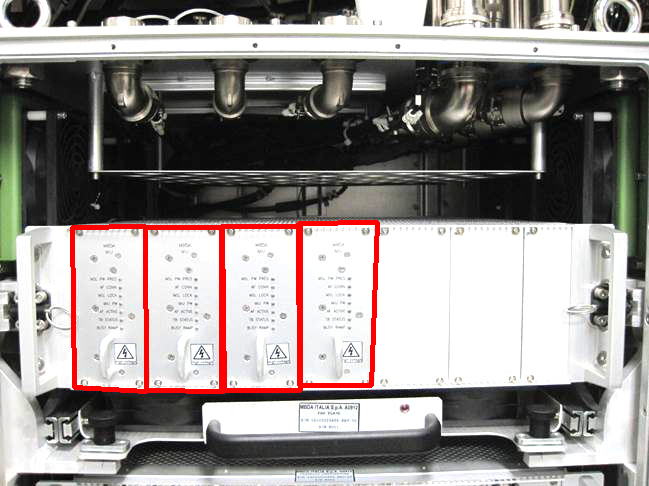
\includegraphics[scale=0.7]{images_not_compressed/intro.png}
				\caption{Application finding 4 patterns from a single training pattern.}
			\end{center}
		\end{figure}
		
		
	
	\chapter{Need}
		\par At work, when people have to make maintenance of the material, they encounter a problem with the density of the maintenance manuals which can make around 700 pages. We try to ease the maintenance by recreating manuals that focuses on the material that the technician is looking at. To obtain this result, we have to analyze the images of the camera and extract the type of material. That is what this report deals with.
		\par This solution can apply to a lot of other objects to find like monuments to extract show the description. \\
		
		\begin{figure}[h]
			\begin{center}
				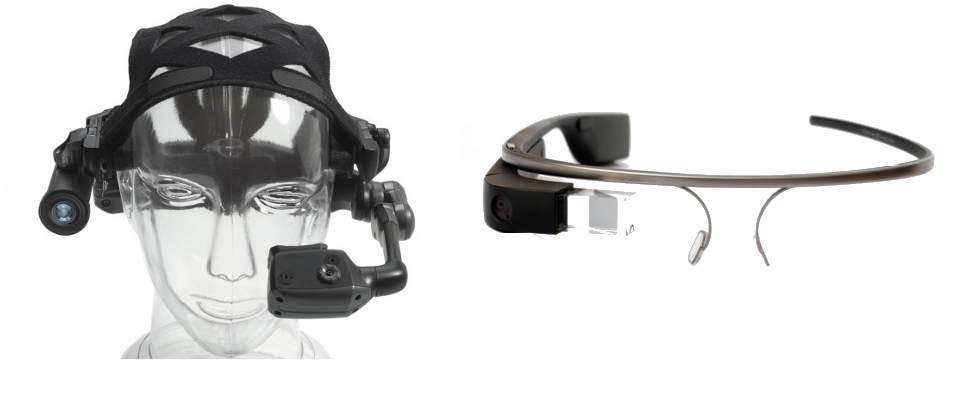
\includegraphics[scale=0.41]{images_not_compressed/helmet.png}
				\caption{type of helmet which the application could be used with}
			\end{center}
		\end{figure}
	
		
	\chapter{Solution}
	\section{Introduction}
	\par To resolve the problem, I only worked on Linux LMDE. It should work on other unix based operating system. For windows it requires Qt3 to open the windows that show the images.
First, I will introduce OpenCV because all the application is based on it. I will talk more precisely about the key points and the descriptors that are computed from them. I will also explain the homography system. All of this component is embedded in the OpenCV library.
Then I will explain how I used them in the explication, how I tested it and what I added to obtain the information about the patterns.
	
	\section{Composants used}
	
	\subsection{OpenCV}
	\begin{wrapfigure}[4]{l}{2cm}
	\vspace{-7mm}
	
\includegraphics[width=2cm]{images_not_compressed/opencv_logo.png}
	\end{wrapfigure}
	\par OpenCV is an image analysis and synthesis library that brings all the necessary for video and photo analysis. Introduced in 2008, it is now used a lot in the fields that require image analysis.
 It is built around a modular system that allows users to install the library in function of their needs.
 Except the non free module, the library is licensed BSD which means that we can reuse and modify all the components freely.
 In this document I will talk more about precise modules of OpenCV like that base and the features2d modules. 
	\subsection[SIFT points]{Scale-Invariant Feature Transform}
	\par SIFT points are points of interest in the image. They precisely the position of an area where all the pixels have approximately the same properties. Using the Laplacian of Gaussian of the image, maxima and minima which correspond to these areas can be extracted.
	\par The biggest advantage of these points is the invariance in transformation like rotation, scaling and translation. Pattern detection algorithm based on this point is insensitive in term of scale and rotation. That is mainly why it has been chosen for this application.
	\par As a result, by the time that the resolution of the pattern is over an acceptable threshold. We can move and rotate the object without altering the detection.
	
	\subsection[Descriptor]{SIFT Descriptor}
	\par The descriptors are computed from the key points. The descriptors associated with the SIFT key points are locally oriented histograms around a SIFT key point \cite{AM}:
	
	\begin{itemize}
			\item We divide space around each key point (x, y) N\ts{2} squares of 4 by 4 \item We compute the gradient \begin{math}G_{x}(a,b,\sigma)\end{math}, \begin{math}G_{y}(a,b,\sigma)\end{math} for the 4 by 4 by N\ts{2} points (a, b)

		\item For each 4 by 4 square, we compute a histogram of the orientations in 8 directions, multiplying by: (1) the module of the gradient (2) the inverse of the distance to the key point (x, y).
 \item To be invariant in rotation: the local orientation of the key point \begin{math} \theta(x,y) \end{math} is used as the origin (null orientation) of the histograms.		
	\end{itemize}

	\par All the key points and the descriptors extracted and computed in the \nameref{constructors} part just after. They are stored in a vector.
	
	
	\subsection{Homography}
	\par  Just to give a simplified idea, the familiar Cartesian plane is composed by a set of points which have a one-to-one correlation to pairs of real numbers, i.e. X-Y on the two axis.\cite{Homography} 
	\par In our case, the points are the key points extracted. By extracting the homography matrix, we can transform the corners of our image to 4 other points representing the position of the object on the scene\cite{TutoHomography}.
	
	\begin{wrapfigure}[12]{r}{10cm}
			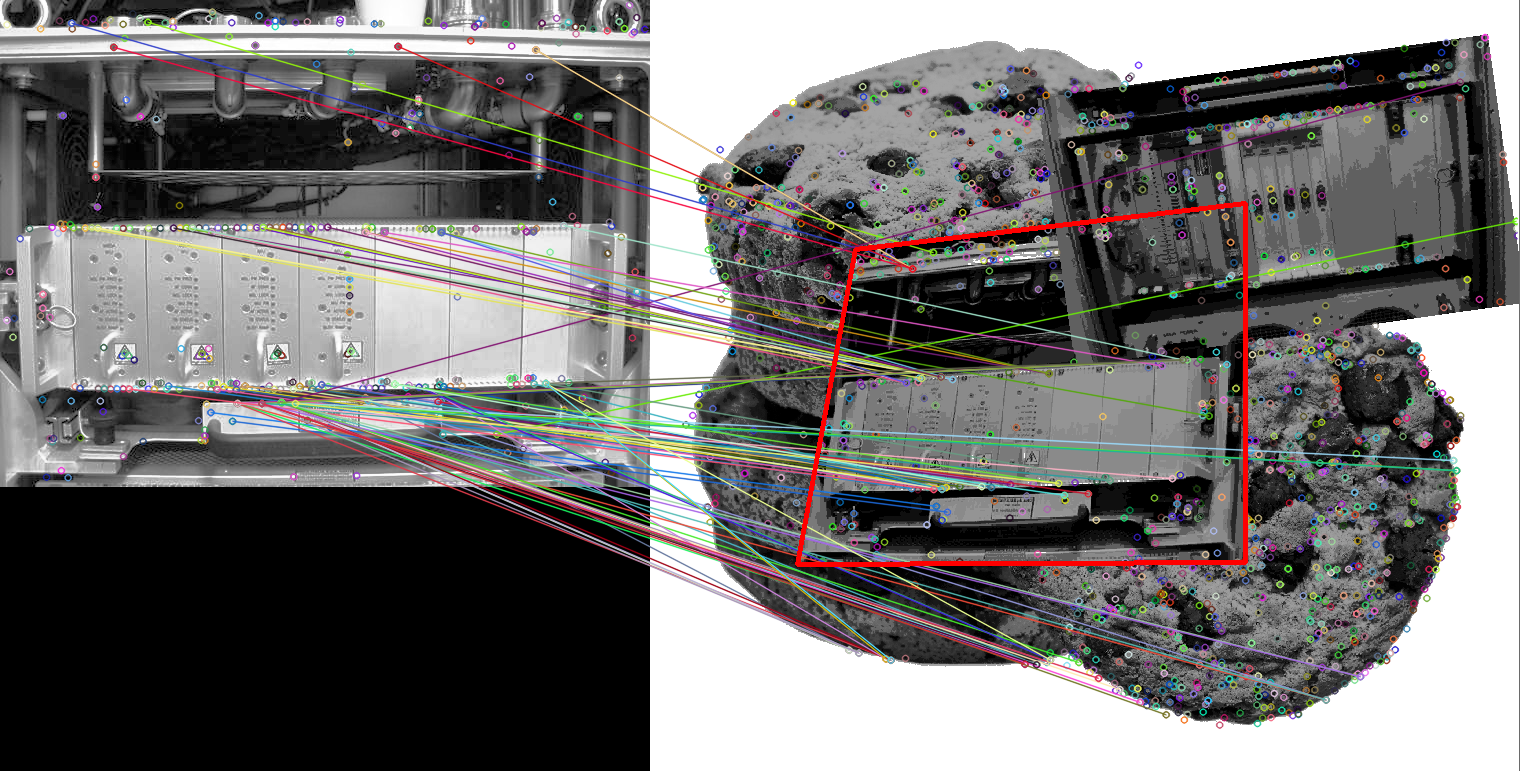
\includegraphics[width=10cm]{images_not_compressed/showHomography.png}
			\caption{Homography with a corner hidden with openCV}
	\end{wrapfigure}
	\par On the image behind we can see that the homography doesn't depend on the corners. All the key points can be a base to analyze the transformation. And using the perspective transform of OpenCV that multiplies the corners by the homography matrix. We obtain the position of the corners on the screen image.
	
	\section{Main functions}
	
	\subsection{Main}
	\par The main idea of the system is to extract all the key points of the scene and all the key points of the pattern in the constructors. Like that you don't have to worry about it in the main program. 
 \par Then you compute the associated descriptors. Both of these containers are implemented in OpenCV and really easy to use. 
 The main loop consists to match the descriptors of the patterns one by one. Comparing them to the scene image we obtain a vector of DMatches that contains the information of each match. That's made by the radius matcher included in OpenCV. 
	\par Then you can perform a homography that uses the descriptors of the matches found to extract an image that looks like the pattern we are looking for. The advantage of this method is the fact that it doesn't depend on the position and the scaling of the image. We also obtain the corners of the object found which allows us to remove the points of interest and descriptors associated from their respective vectors. That method avoids recomputing all the key points and descriptors which is very expensive in resources. 
	\par To stop the loop there are 2 options. First, there is not enough match between the two images. Secondly the number of key values removes after finding a pattern is too low. In both cases the match is not drawn on the image and the next pattern to analyze is set.
	\subsection{Constructors}
	\label{constructors}
	\subsubsection{Scene}
	\par The scene represents the vision of the camera and the current position of its analysis.
It requires only the location of the image to be built. It sets the key points and computes the descriptors.
\par It uses a SiftFeatureDector from OpenCV with a minHessian (exigence of the detector) value of 10000. It is a very high value but the tests show me that more this value is high, better are the results\footnote{It also depends on the pattern minhessian value} and the quality of the image itself.
	
	\subsubsection{Pattern}
	\par A pattern represents an object that you want to be recognized in the image. It has simple attributes like a name and a matrix corresponding to the image it represents. But it also has more complex attributes like the vector of key points that we extract in the constructor\footnote{It can also be stored in a file}, the matrix of descriptor that represents the properties of each point and the thresholds. The thresholds are separated in two different attributes, the munition that we told about just before in the scene section and the threshold properly spoken. The second one refers to the radius matching system, it is the maximum acceptable distance between two descriptors during the matching process. There is no universal value so we use values between 150 to 300 that we have to test one by one to see which one gives the best results.
 \par The program contains a little part of code that brings the possibility to try different values quickly.
	
	
	\subsubsection{Corners}
	\par Corners is a simple class containing 4 "point2d" (x, y point implementation from OpenCV).
It also contains a method that determines if the point is inside the polygon represented by the corners. It uses the fact that a point is inside a polyline if a line drawn from the point to the infinity cross odd number of segments.
	\begin{figure}[h]
		\begin{center}
			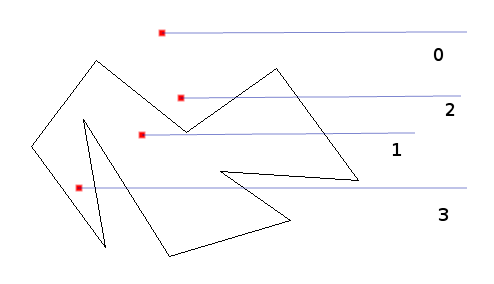
\includegraphics[scale=0.7]{images_not_compressed/isIn.png}
			\caption{Illustation of the method to determin if a point is inside a polyline}
		\end{center}
	\end{figure}
		
	
	
	

	\listoffigures

	\bibliography{/home/manu/workspace/Scanner/Report/biblio}{}
	\bibliographystyle{plain}
	
\end{document}